\subsection{Einfluss der Messmethode (Reflexion/Transmission) \label{sec:einflussmethode}}

Als erstes werden die gemessenen Transmissions- und Reflexionsverläufe sowohl für die Messungen mit variabler Konzentration als auch für die Messungen mit variabler Rotationsgeschwindigkeit in Abb.~\ref{fig:rpm_spektren} graphisch dargestellt. 

Bei den Spektren mit variabler Konzentration in Abb.~\ref{fig:conc_spektren} fällt direkt auf, dass die Transmissionsspektren deutlich verrauschter als die Reflektionsspektren sind. Beide Spektren zeigen bei höhrerer Konzentration der PS-Kugeln eine deutliche Abnahme des Abstands zwischen den einzelnen Maxima, bei niedrigen Konzentrationen lassen sich überhaupt keine Maxima im Wellenlängenbereich mehr ausmachen. Dies lässt direkt auf eine steigende Filmdicke bei höherer Konzentration schließen, da erhöhte Reflexion in der Schicht zu verstärkter Interfernz führt.

Bei unterschiedlicher Rotationsgeschwindigkeit in Abb.~\ref{fig:rpm_spektren} sieht man bei steigender Rotationsgeschwindigkeit bei beiden Messmethoden eine Abnahme der Peaks im gemessenen Wellenlängenbereich bzw.~eine Zunahme der Abstände der Peaks. Auch hier sind die Transmissionsspektren etwas verrauschter als die Relektionsspektren, jedoch weit weniger als bei den Messungen mit variabler Konzentration. Aus beiden Spektren lässt sich hier ablesen, dass die Schichtdicke bei steigener Geschwindigkeit wohl abnimmt.

\begin{figure}[h!]
    \centering
    \begin{subfigure}{.5\textwidth}
      \centering
      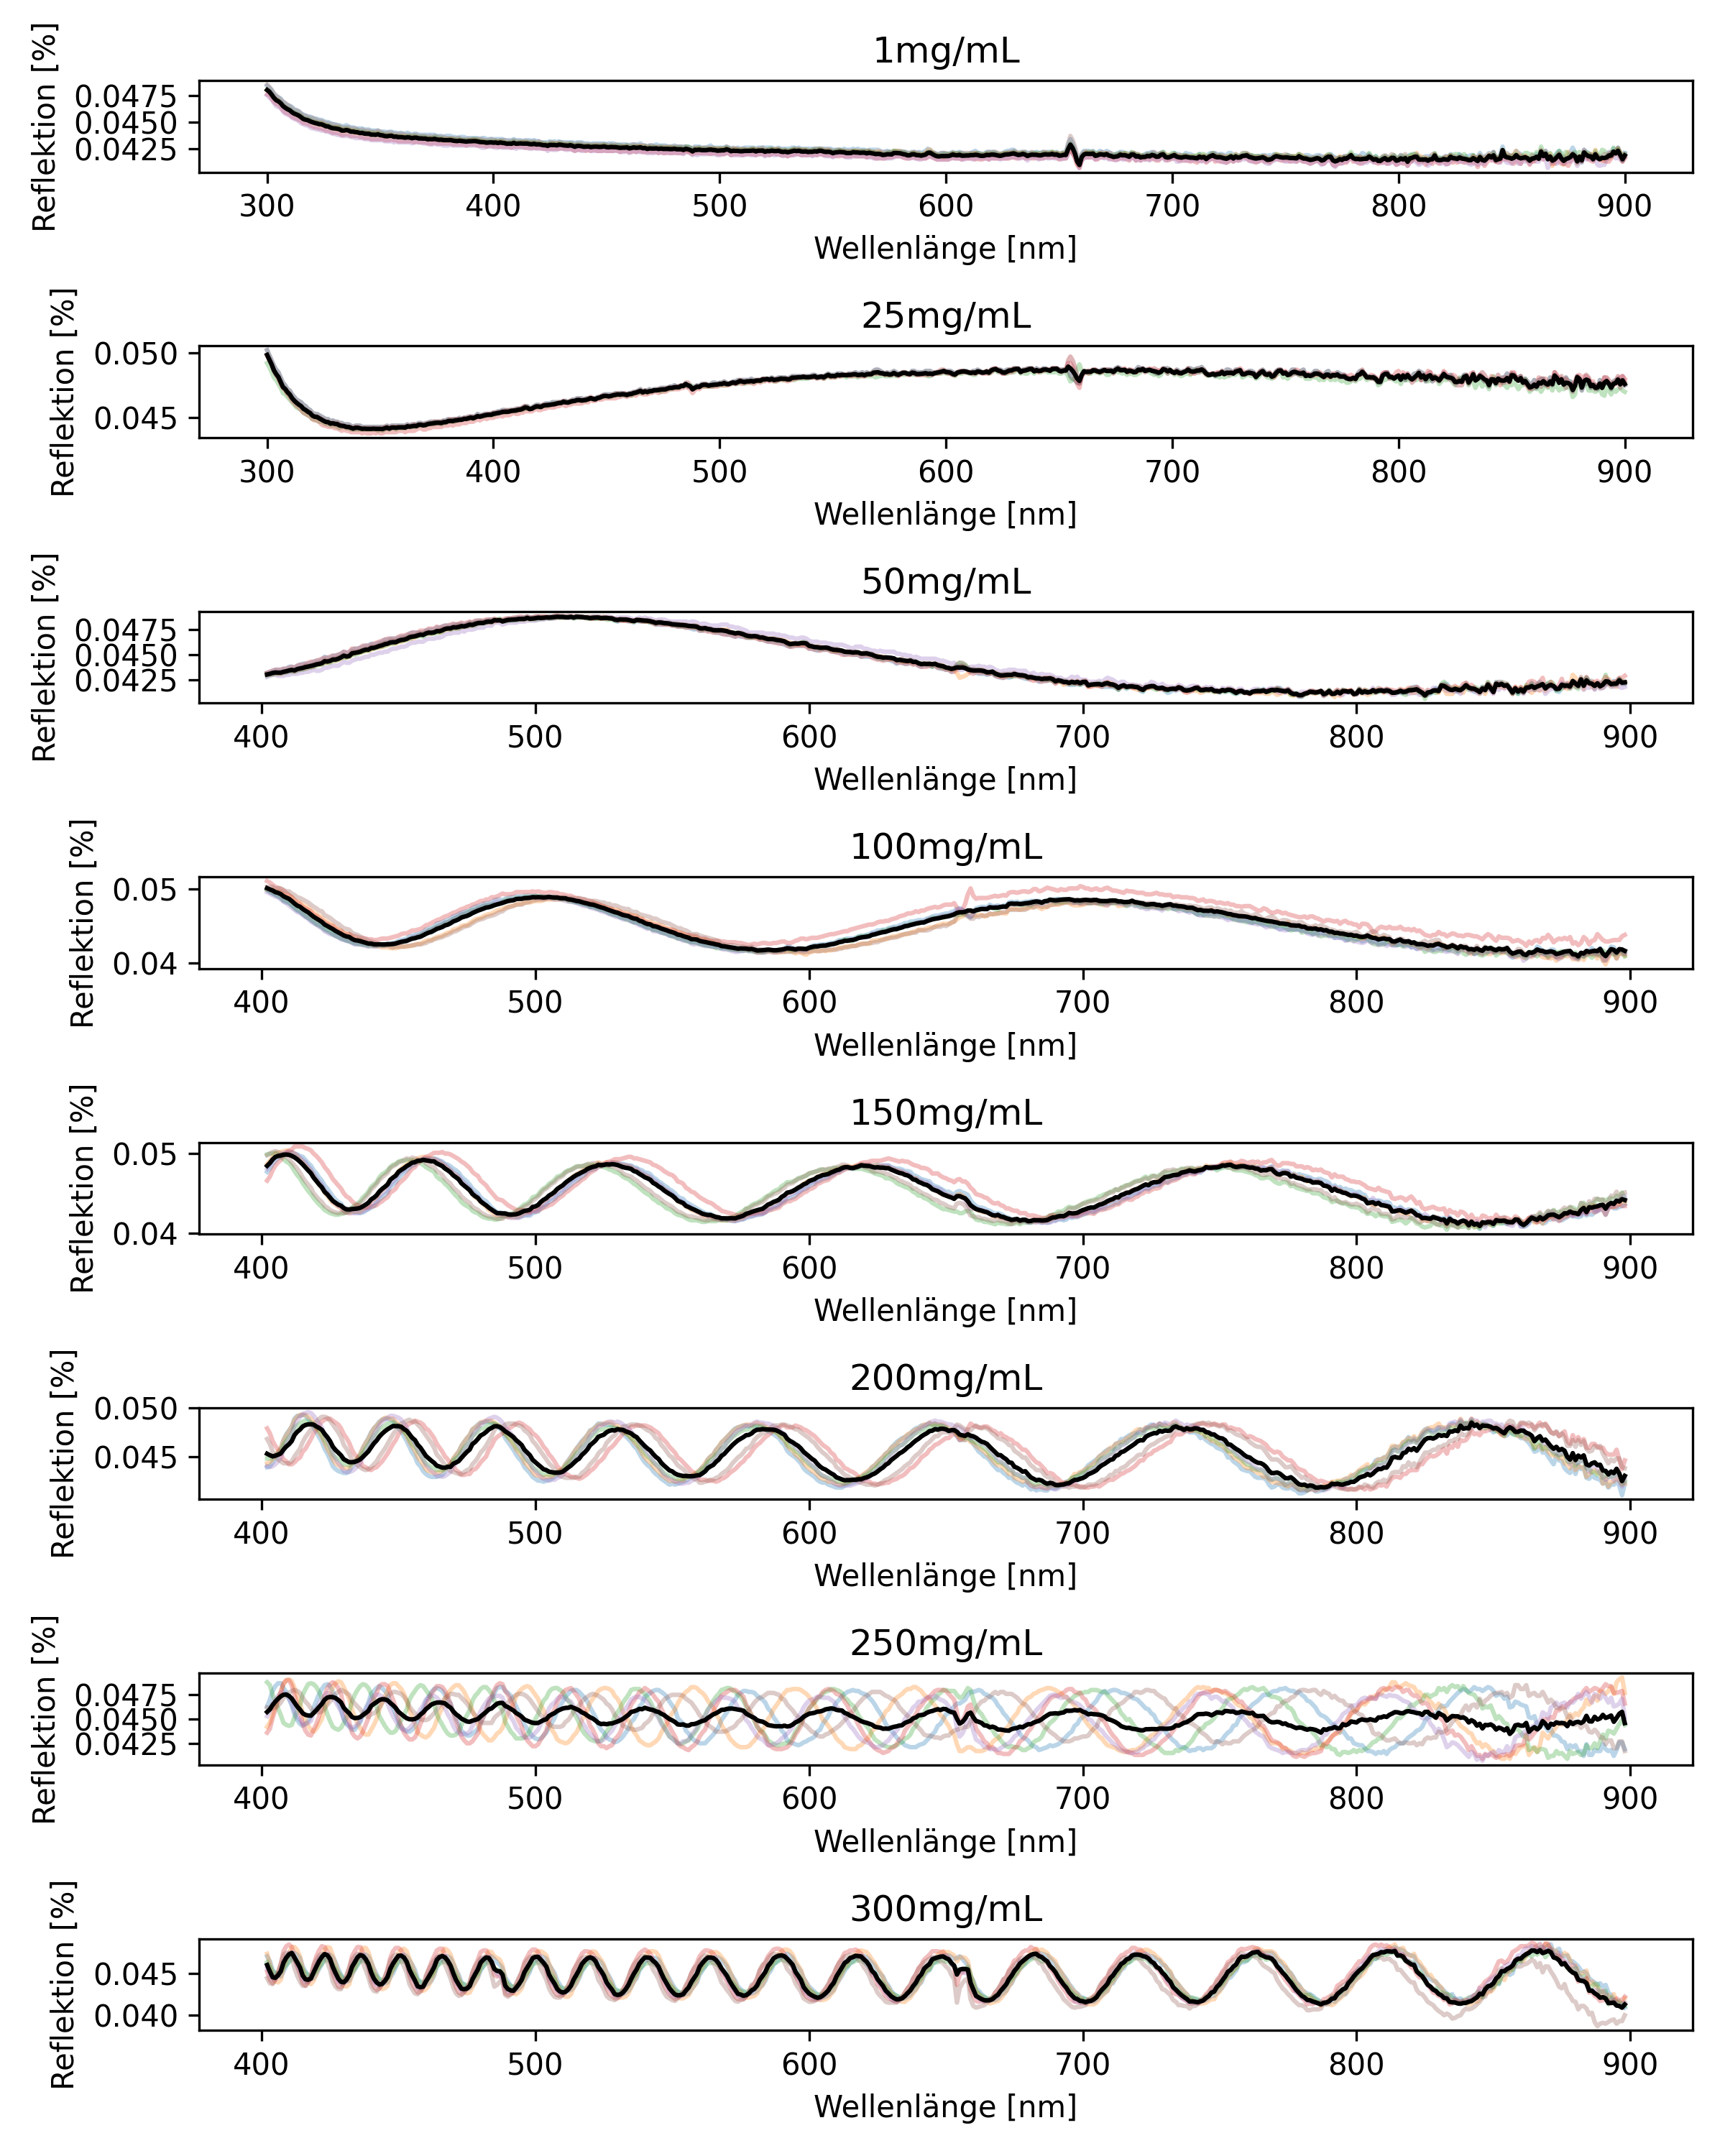
\includegraphics[width=.8\linewidth]{refl_conc.png}
      \caption{Reflektionsspektren}
      \label{fig:refl_conc}
    \end{subfigure}%
    \begin{subfigure}{.5\textwidth}
      \centering
      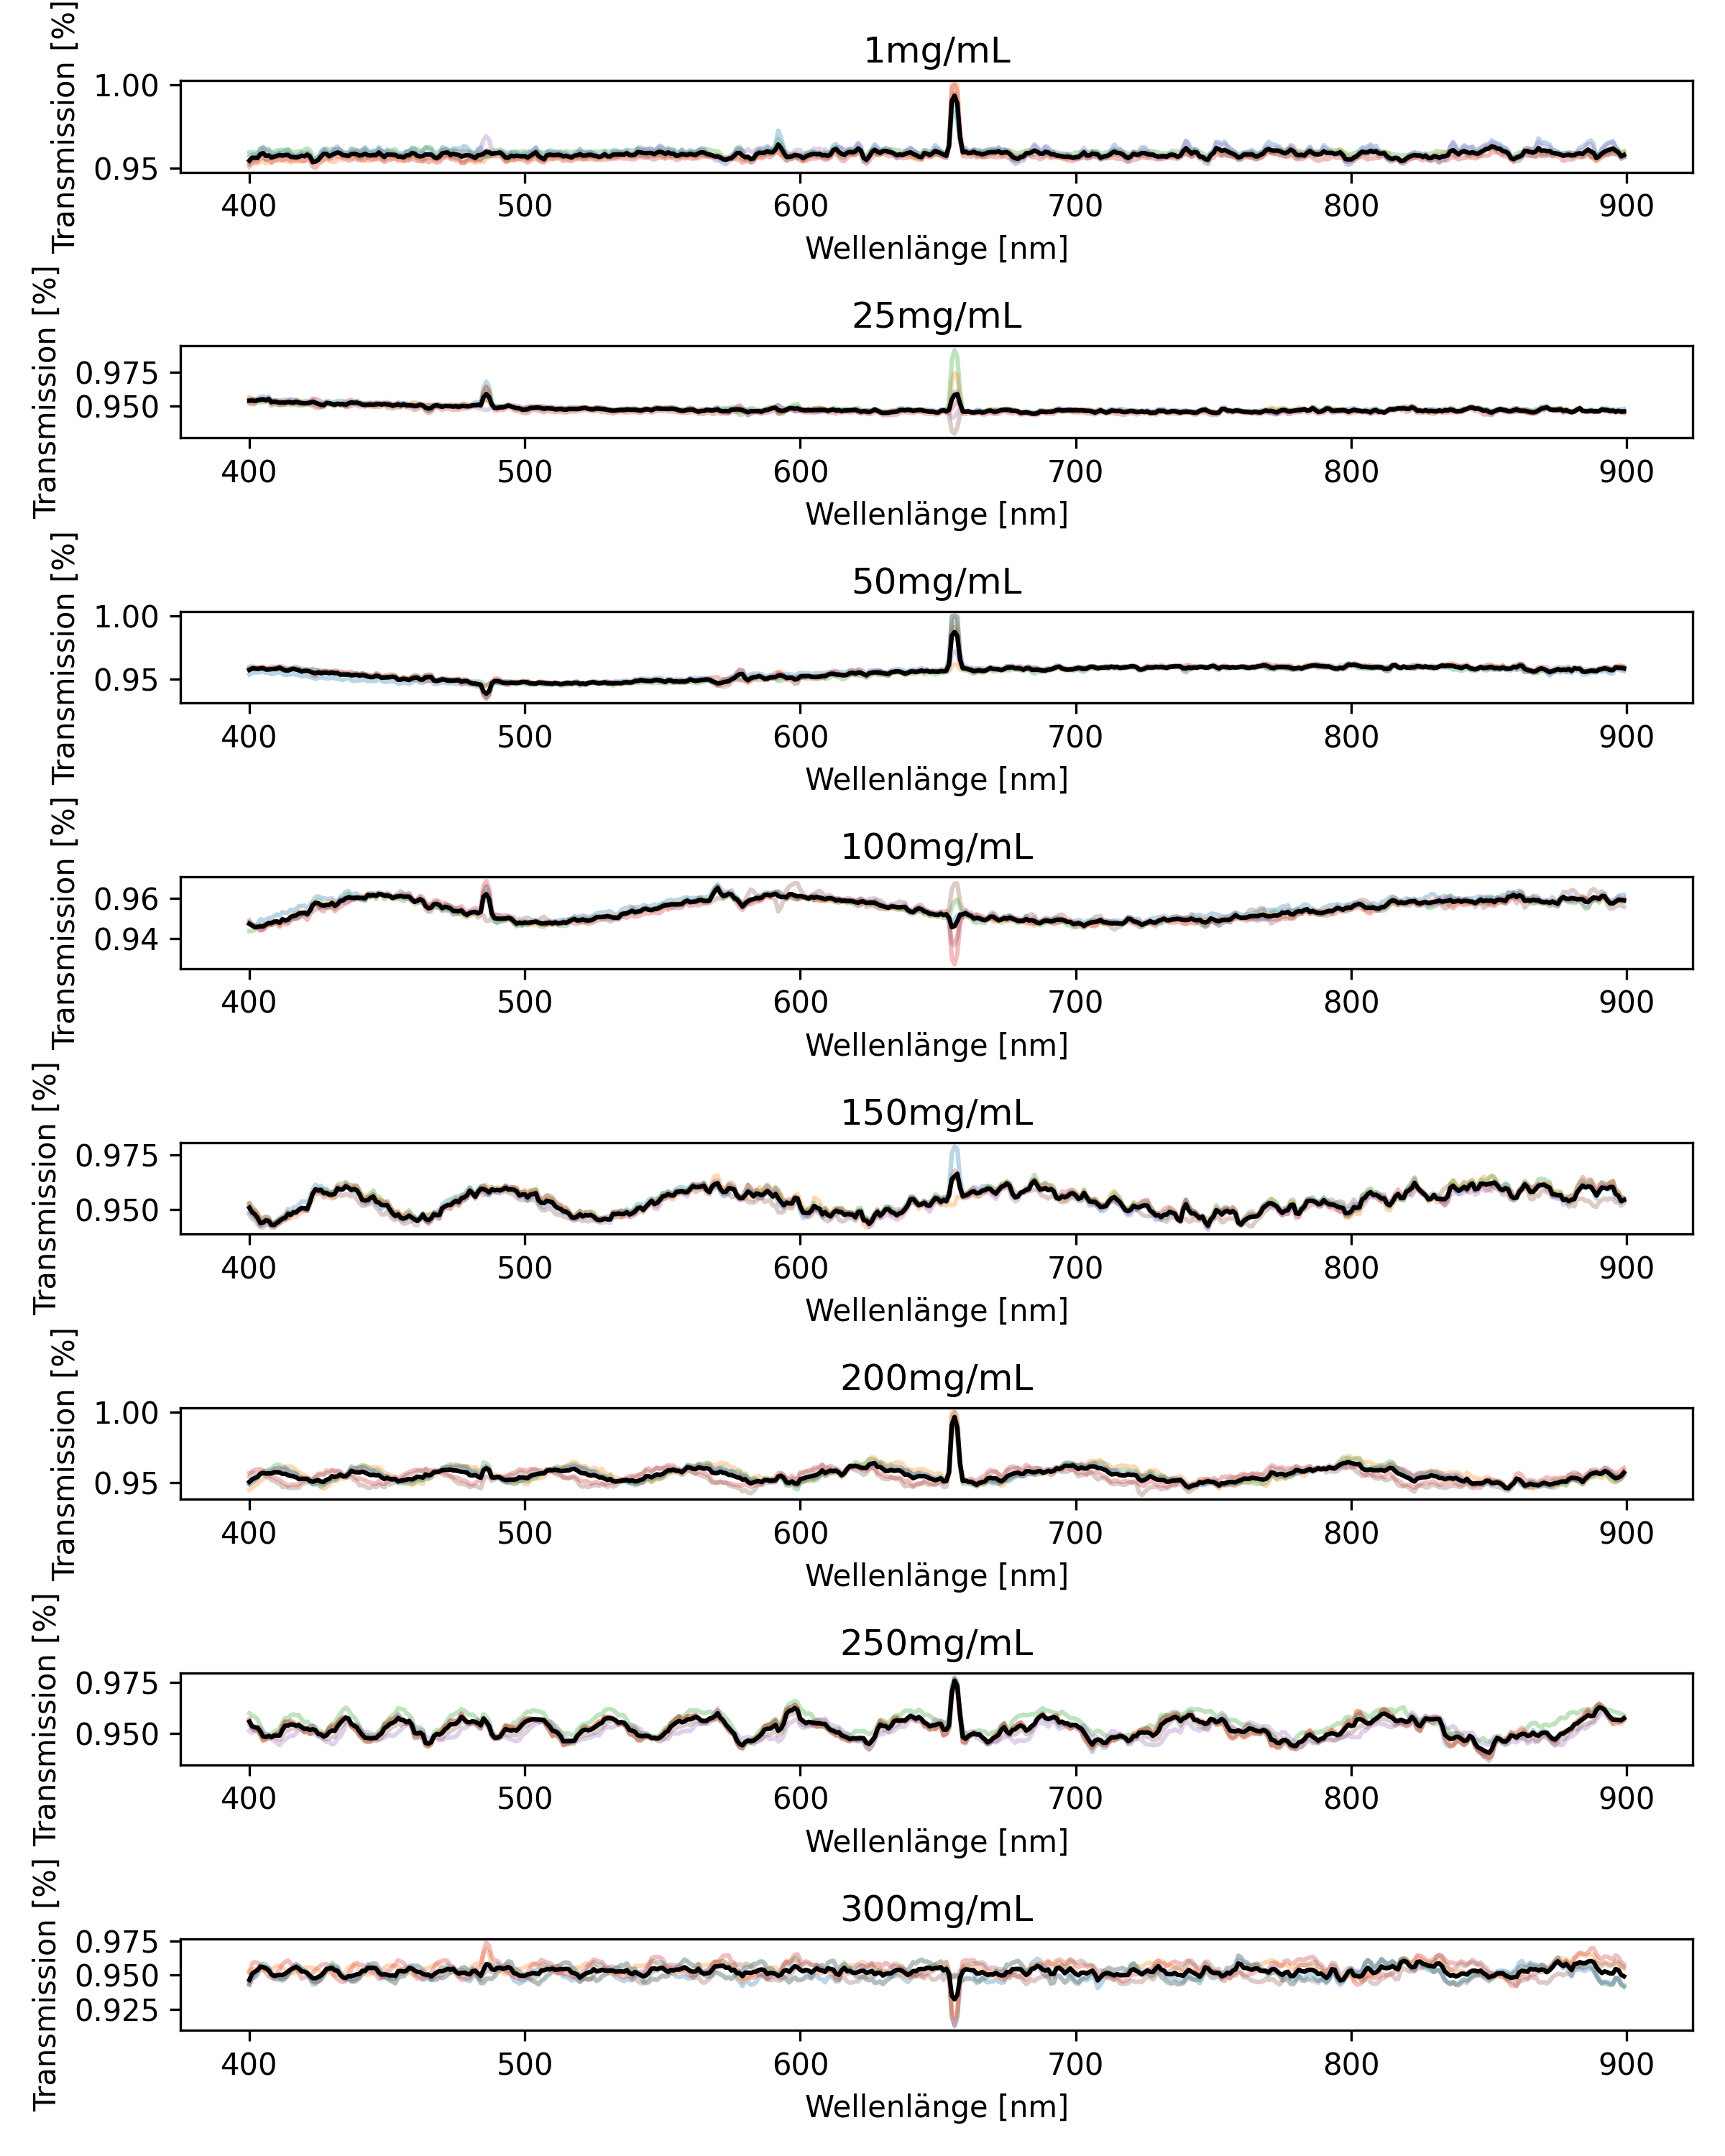
\includegraphics[width=.8\linewidth]{trans_conc.png}
      \caption{Transmissionsspektren}
      \label{fig:refl_trans}
    \end{subfigure}
    \caption{Geplottete Spektren für die Messungen mit variabler Konzentration. Jede Messreihe besteht aus 6 Einzelmessungen, die farbig dargestellt sind. Zur bessereren Übersichtlichkeit wird zusätzlich der jeweilige Mittelwert in schwarz geplottet.}
    \label{fig:conc_spektren}
\end{figure}

\begin{figure}[h!]
    \centering
    \begin{subfigure}{.5\textwidth}
      \centering
      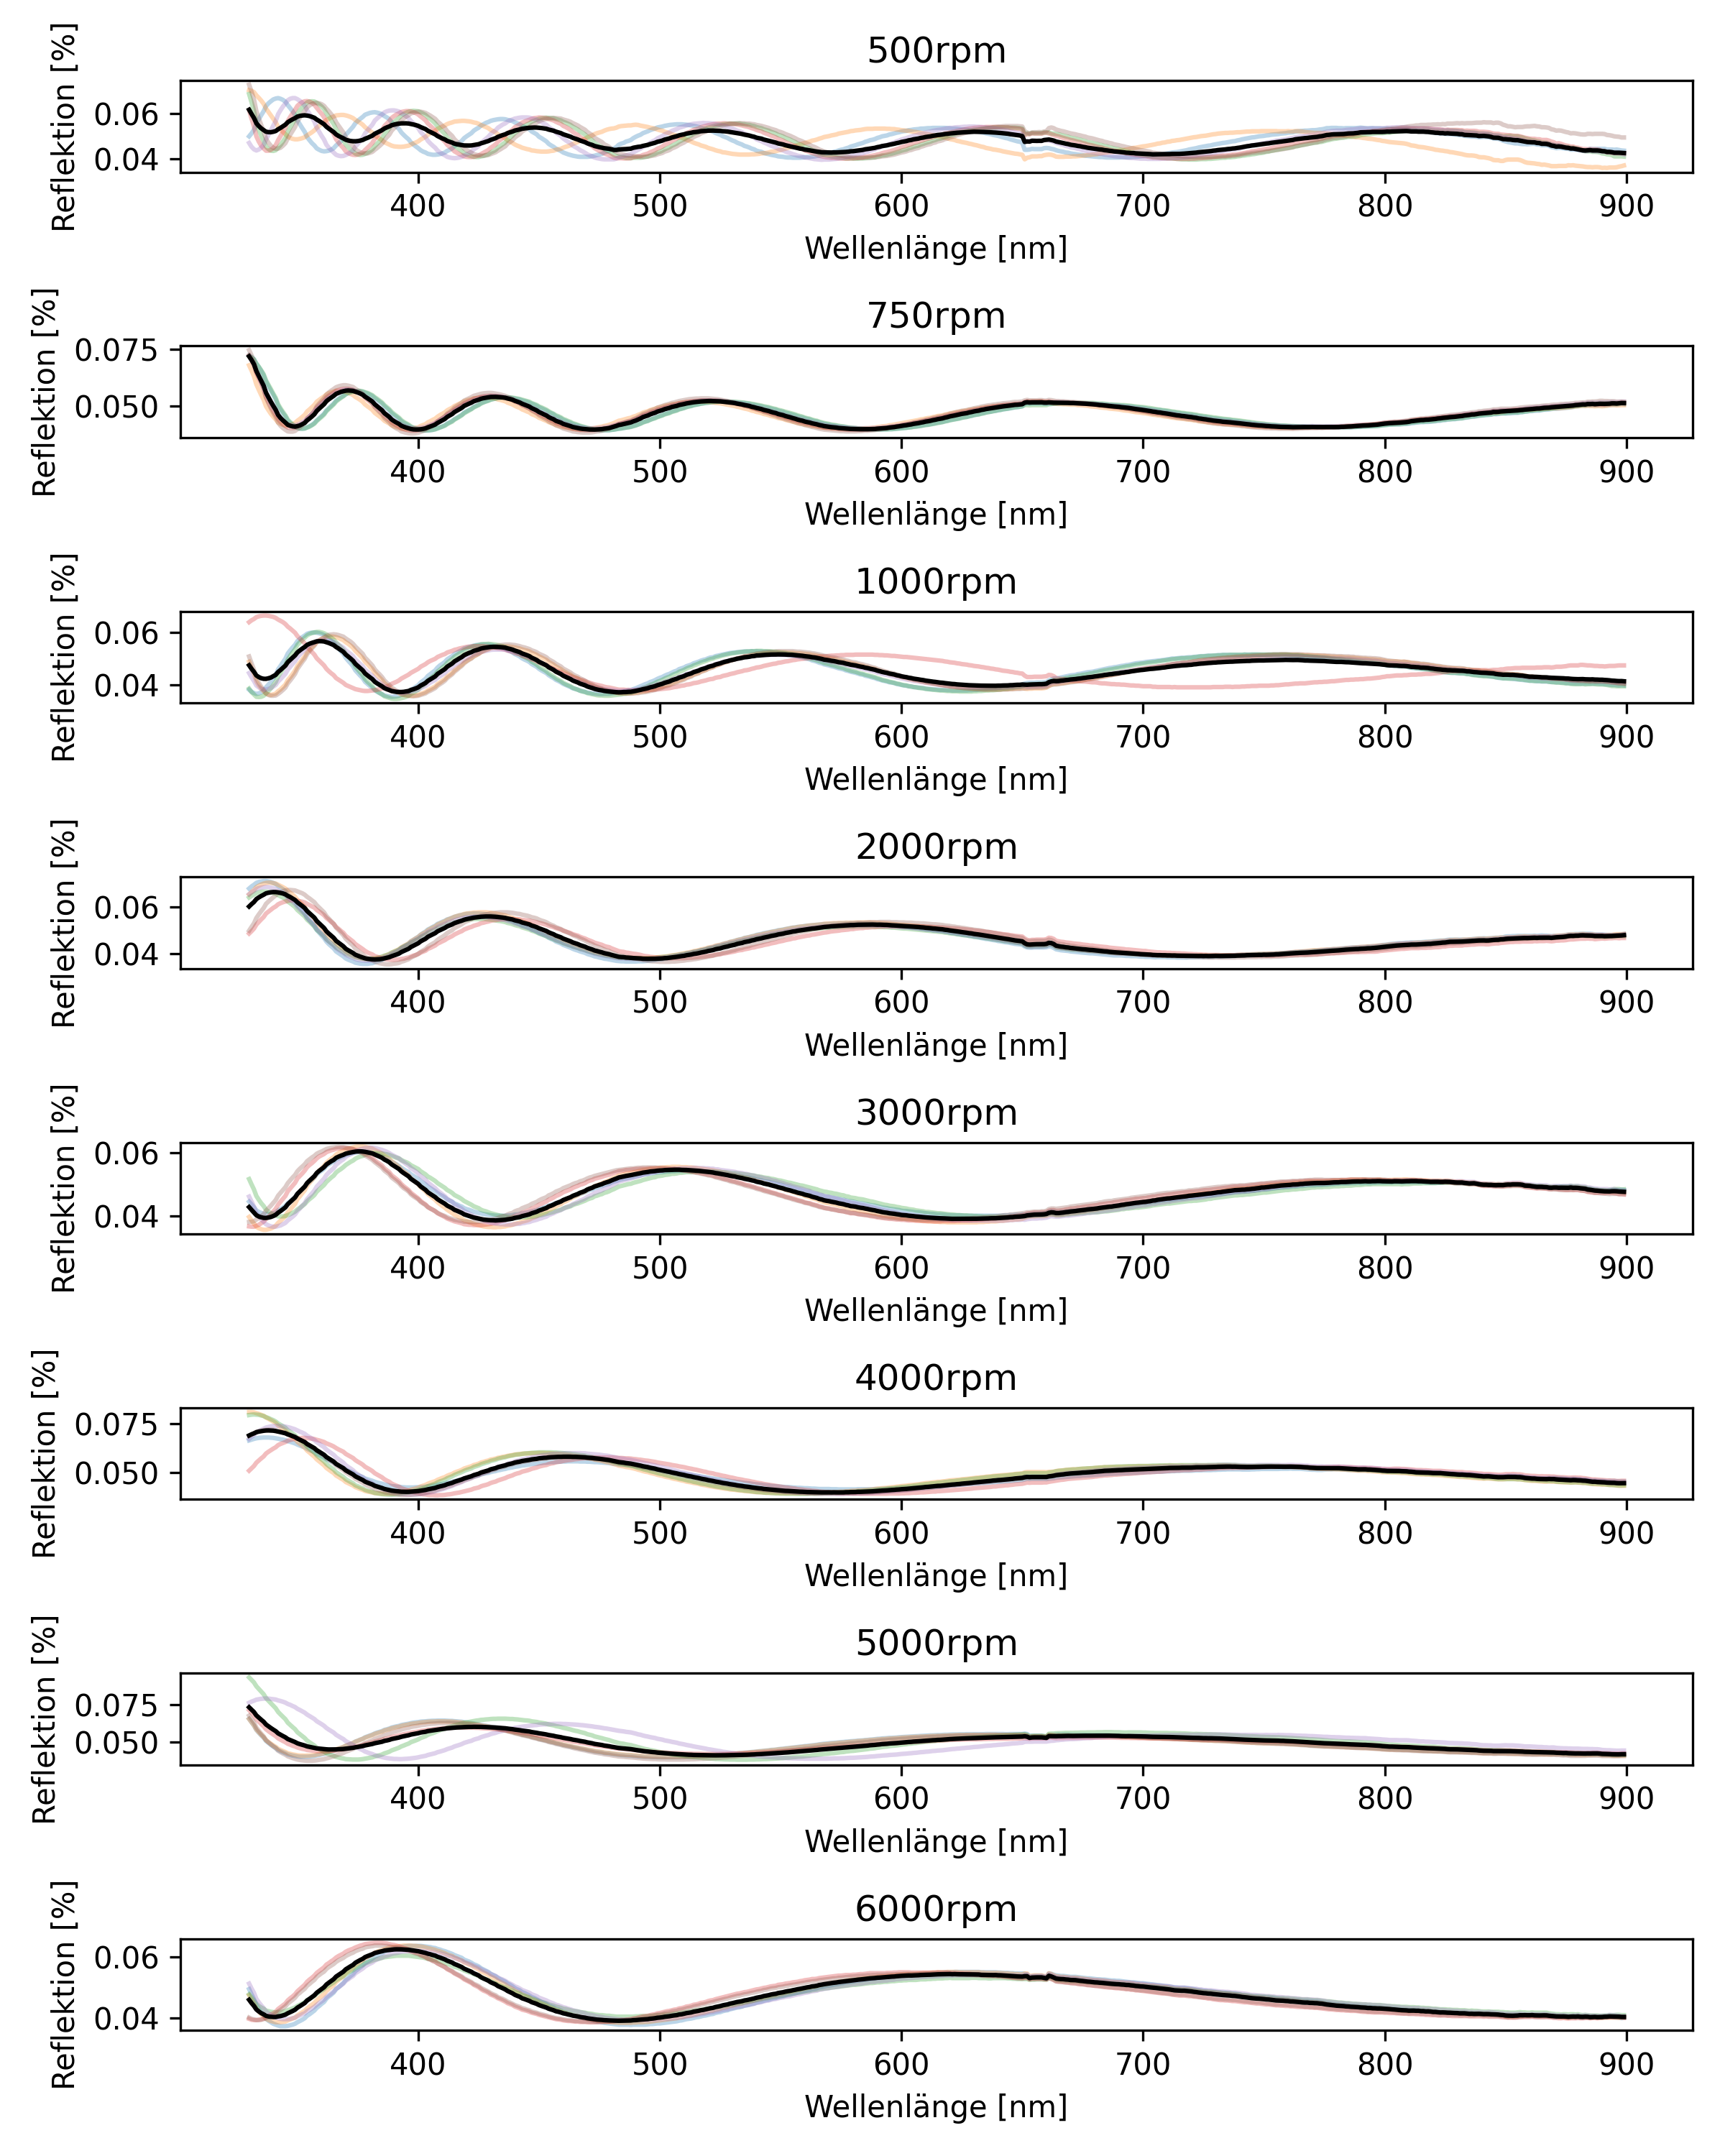
\includegraphics[width=.8\linewidth]{refl_rpm.png}
      \caption{Reflektionsspektren}
      \label{fig:refl_rpm}
    \end{subfigure}%
    \begin{subfigure}{.5\textwidth}
      \centering
      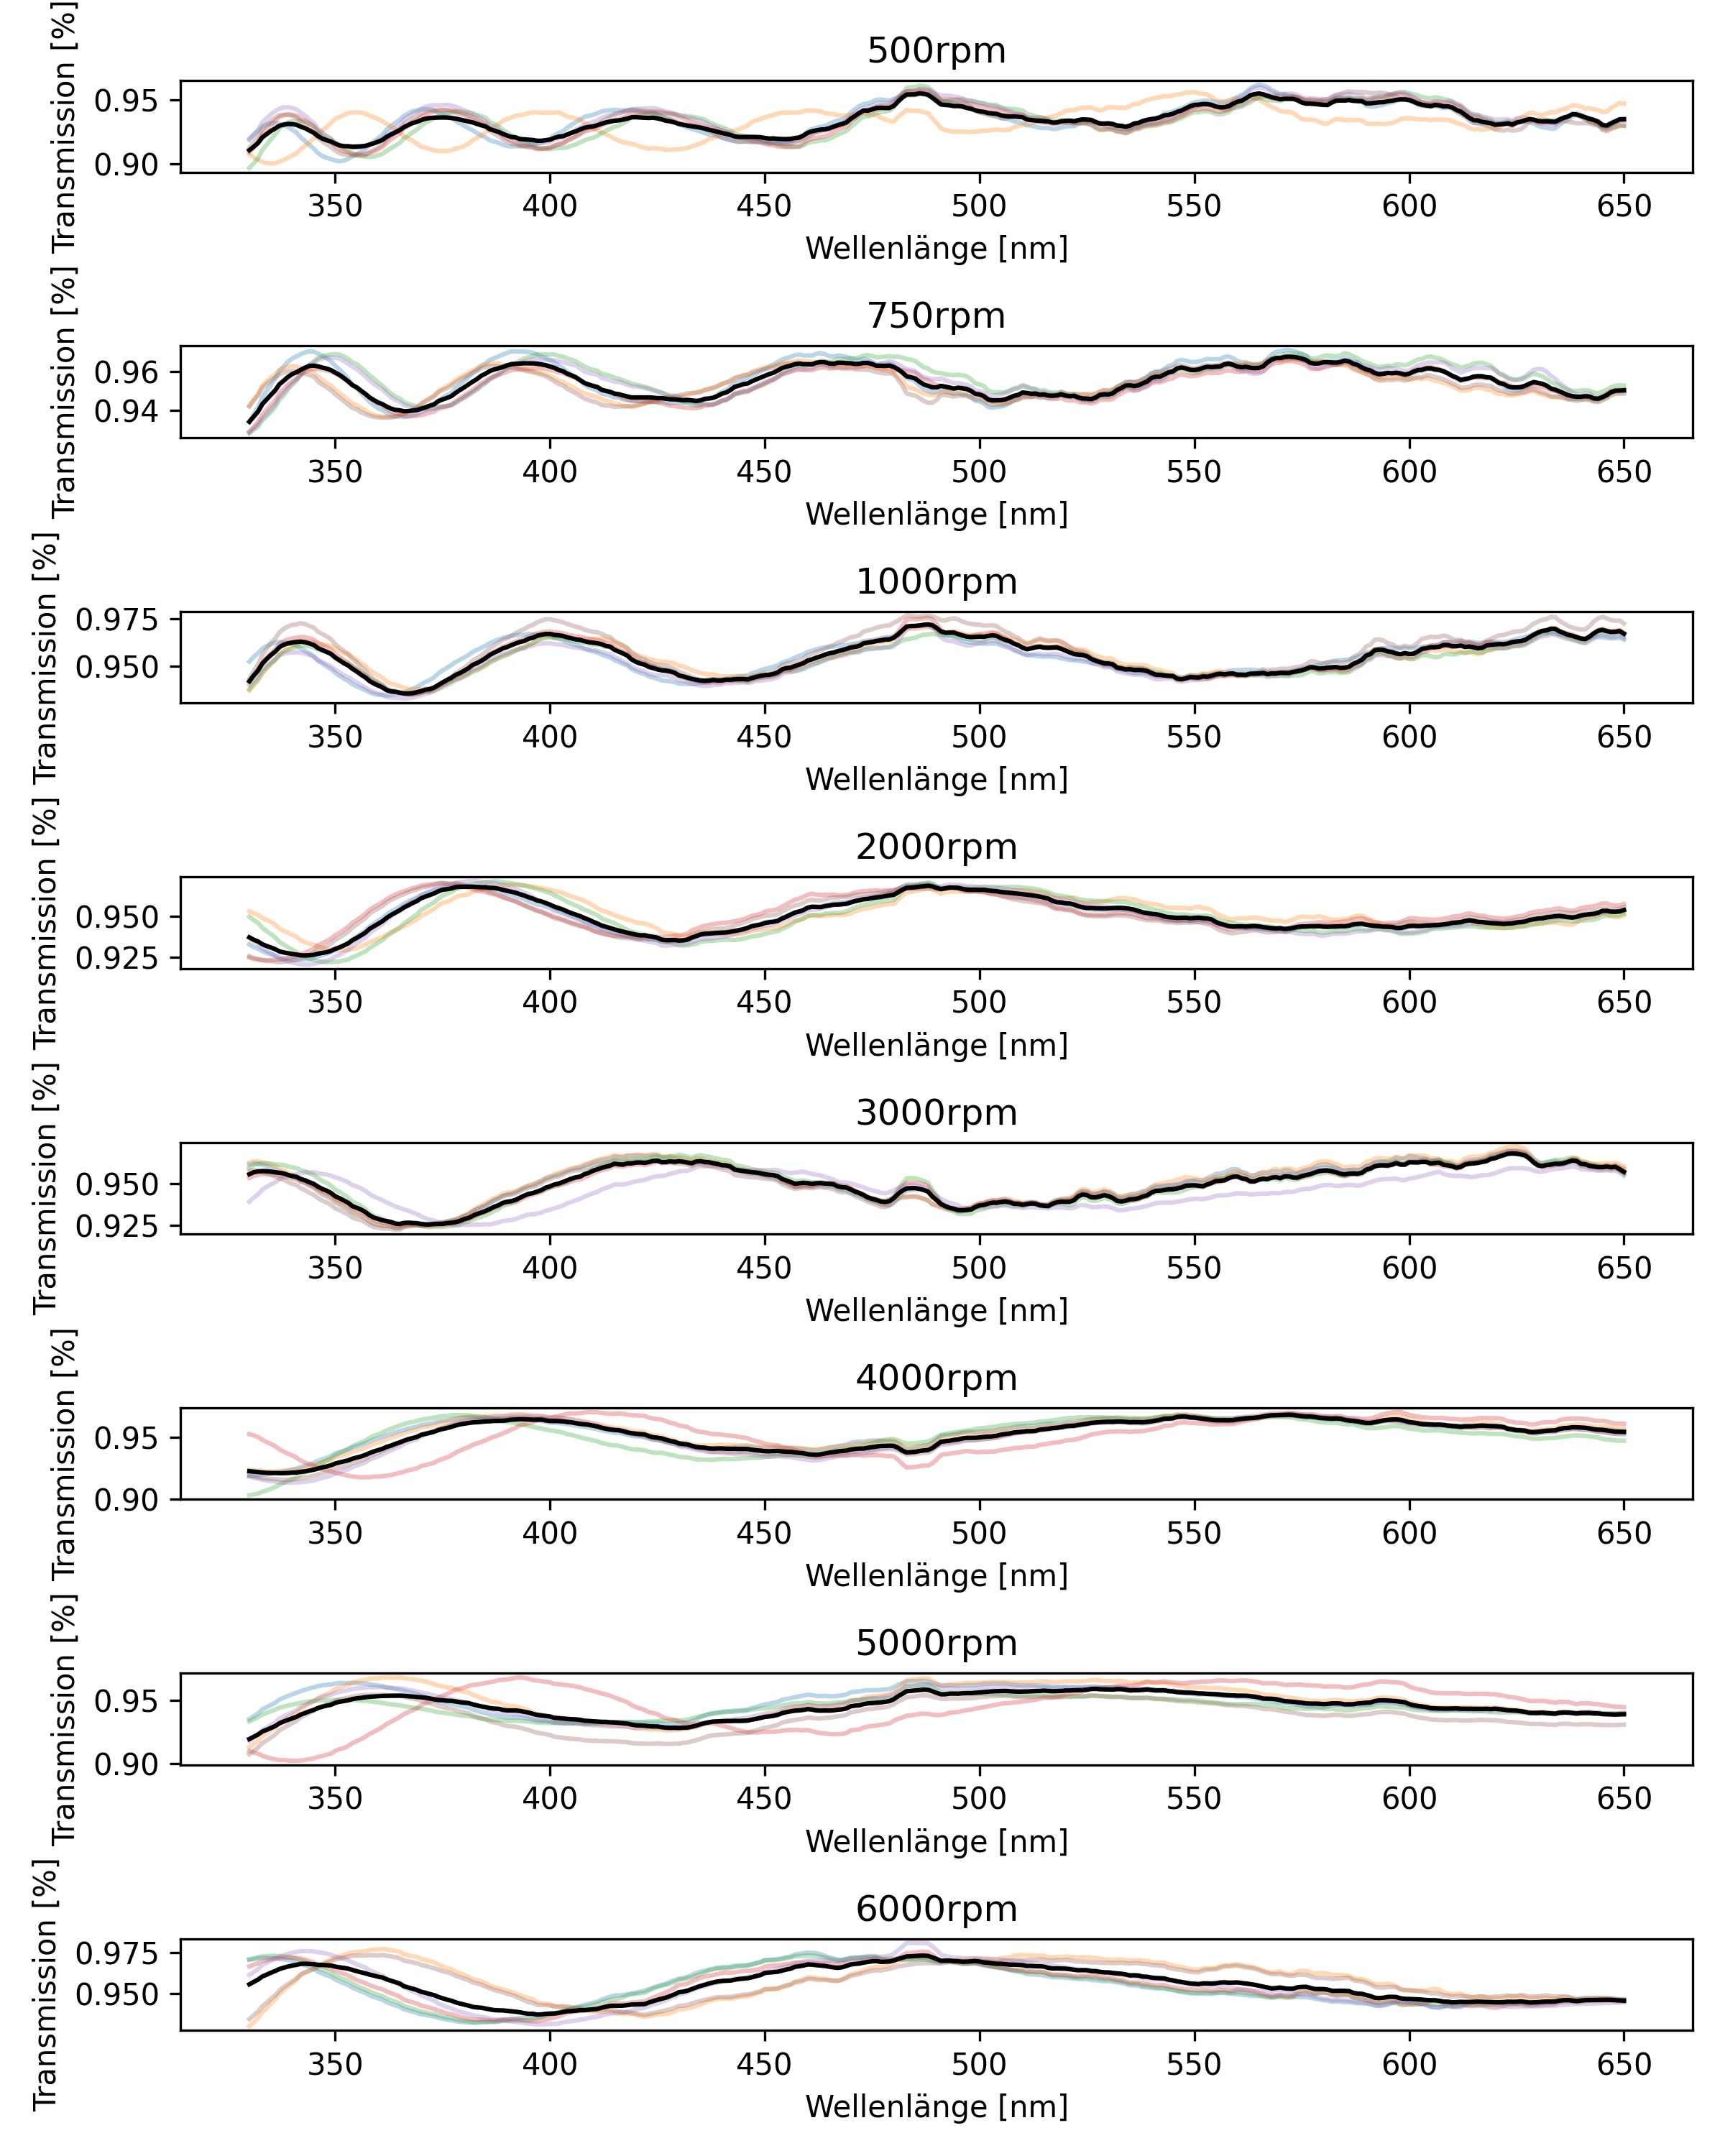
\includegraphics[width=.8\linewidth]{trans_rpm.png}
      \caption{Transmissionsspektren}
      \label{fig:trans_rpm}
    \end{subfigure}
    \caption{Geplottete Spektren für die Messungen mit variabler Rotationsgeschwindigkeit. Jede Messreihe besteht aus 6 Einzelmessungen, die farbig dargestellt sind. Zur bessereren Übersichtlichkeit wird zusätzlich der jeweilige Mittelwert in schwarz geplottet.}
    \label{fig:rpm_spektren}
\end{figure}

Um die bisher qualitativ gewonnenen Erkenntnisse zu überprüfen, werden nun für jede Probe die Schichtdicken und die Heterogenität, die als Maß für die Homogenität der Proben benutzt werden kann, bestimmt. Die Messung an jeder Probe wurde sowohl für die Reflektionsspektren als auch für die Transmissionsspektren an 6 verschiedenen Stellen durchgeführt, weshalb als Filmdicke der Mittelwert der 6 Einzelmessungen der Dicke genommen wird. Die Heterogenität $h$ der Probe berechnet sich dann wie folgt:
\begin{equation}
    h = \frac{<d>}{std(d)}
\end{equation}
mit $<d>$ dem Mittelwert der Schichtdicke $d$ und $std(d)$ der Standardabweichung der Dicke. Die Heterogenität steigt mit zunehmender Homogenität der Probe, da für eine homogene Probe die Standardabweichung klein und $h$ dadurch groß wird. 

\begin{table}[h!]
\centering
\begin{tabular}{|c|c|c|c|c|c|c|c|c|}
    \hline
    \makecell{Drehzahl\\in $rpm$} & \makecell{$<d_R>$\\in nm} & \makecell{$<d_T>$\\in nm} & \makecell{$std(d_R)$\\in nm} & \makecell{$std(d_T)$\\in nm} & $h_R$ & $h_T$ & $\chi_R$ & $\chi_T$ \\ [0.5ex]
    \hline \hline
   500 & 894,55 & 904,45 &31,64 & 21,78 & 28,28 & 41,54 & 0,045379 & 0,140883 \\
   750 & 740,48 & 729,07& 8,95 & 9,71 & 82,70 & 75,08 & 0,066360 & 0,113425 \\
   1000 & 604,60 & 614,60 & 5,87 & 4,96 & 103,05 & 123,91 & 0,085911 & 0,112254 \\
   2000 & 466,72 & 466,17 & 7,46 & 9,21 & 62,53 & 50,63 & 0,062833 & 0,068316 \\
   3000 & 405,22 & 397,17 & 7,88 & 7,43 & 51,45 & 53,44 & 0,067570 & 0,029994 \\
   4000 & 360,85 & 359,40 & 8,20 & 10,33 & 44,02 & 34,80 & 0,044741 & 0,061081 \\
   5000 & 329,67 & 329,73 & 16,35 & 15,84 & 20,16 & 20,82 & 0,037299 & 0,039006 \\
   6000 & 302,68 & 312,10 & 5,83 & 12,33 & 51,90 & 25,32 & 0,044481 & 0,131909 \\ [1ex]
   \hline
   \end{tabular}
   \caption{Mittelwert der Filmdicke $<d>$, Standardabweichung $std(d)$, Heterogenität $h$ und Fitgüte $X$ für die Messungen mit variabler Rotationsgeschwindigkeit.}
   \label{tab:rpm_val}
\end{table}

\begin{table}[h!]
    \centering
    \begin{tabular}{|c|c|c|c|c|c|c|c|c|}
        \hline
        \makecell{Konzentration\\in $\si{\milli\gram\per\milli\litre}$} & \makecell{$<d_R>$\\in nm} & \makecell{$<d_T>$\\in nm} & \makecell{$std(d_R)$\\in nm} & \makecell{$std(d_T)$\\in nm}& $h_R$ & $h_T$ & $\chi_R$ & $\chi_T$ \\ [0.5ex]
        \hline \hline
        1 & 6,23 & 6,12 & 1,31 & 6,97 & 4,75 & 0,88 & 0,000158 & 0,012661 \\
        25 & 101,67 & 140,68 & 0,52 & 8,35 & 196,88 & 16,85 & 0,130681 & 0,033684 \\
        50 & 249,02 & 242,53 & 2,33 & 5,52 & 107,06 & 43,95 & 0,076064 & 0,056423 \\
        100 & 538,12 & 546,57 & 2,97 & 3,89 & 180,93 & 140,48 & 0,077935 & 0,064551 \\
        150 & 1067,67 & 1069,78 & 12,97 & 4,98 & 82,33 & 214,72 & 0,087111 & 0,055296 \\
        200 & 1741,27 & 1758,75 & 17,24 & 22,85 & 100,99 & 76,96 & 0,092777 & 0,102557 \\
        250 & 2841,97 & 2827,73 & 98,44 & 13,90 & 28,87 & 203,44 & 0,097175 & 0,057670 \\
        300 & 3980,67 & 3944,95 & 12,46 & 97,12 & 319,45 & 40,62 & 0,103426 & 0,062149 \\[1ex]
       \hline
       \end{tabular}
       \caption{Mittelwert der Filmdicke $<d>$, Standardabweichung $std(d)$, Heterogenität $h$ und Fitgüte $X$ für die Messungen mit variabler Konzentration.}
       \label{tab:conc_val}
    \end{table}

In den Tabellen \ref{tab:rpm_val} und \ref{tab:conc_val} sind die berechneten Werte für die Filmdicke, die Standardabweichung, die Heterogenität und die Fitgüte für die Messungen mit variabler Rotationsgeschwindigkeit und variabler Konzentration aufgelistet. Die Fitgüte $\chi$ ist hierbei ein Maß für die Güte des Fits der gemessenen Spektren mit den theoretischen Spektren. Je kleiner der Wert, desto besser ist der Fit.
Bei beiden Messreihen liegen die Mittelwerte der Schichtdicken für beide Messmethoden in einem ähnlichen Bereich. Bei den Messungen mit unterschiedlicher Rotationsgeschwindigkeit lässt sich dies auch für die Standardabweichungen und Heterogenität sagen, bei den konzentrationsvarrierten Messungen gibt es jedoch sehr große Abweichungen bei den beiden Größen. Insgesamt kann man also sagen, dass unsere Proben sehr unterschiedlich homogen sind, wobei es auch eher unhomogene Proben zu geben scheint.
Es ist kein klarer Trend erkennbar, ob die Reflektions- oder Transmissionsmessung zu besseren Ergebnissen führt. Dies bestätigt sich auch bei einem Plot der Fitgüte gegen die Schichtdicke für beide Messreihen, dargestellt in Abb.~\ref{fig:guete_spektren}.



\begin{figure}[h!]
  \centering
  \begin{subfigure}{.4\textwidth}
    \centering
    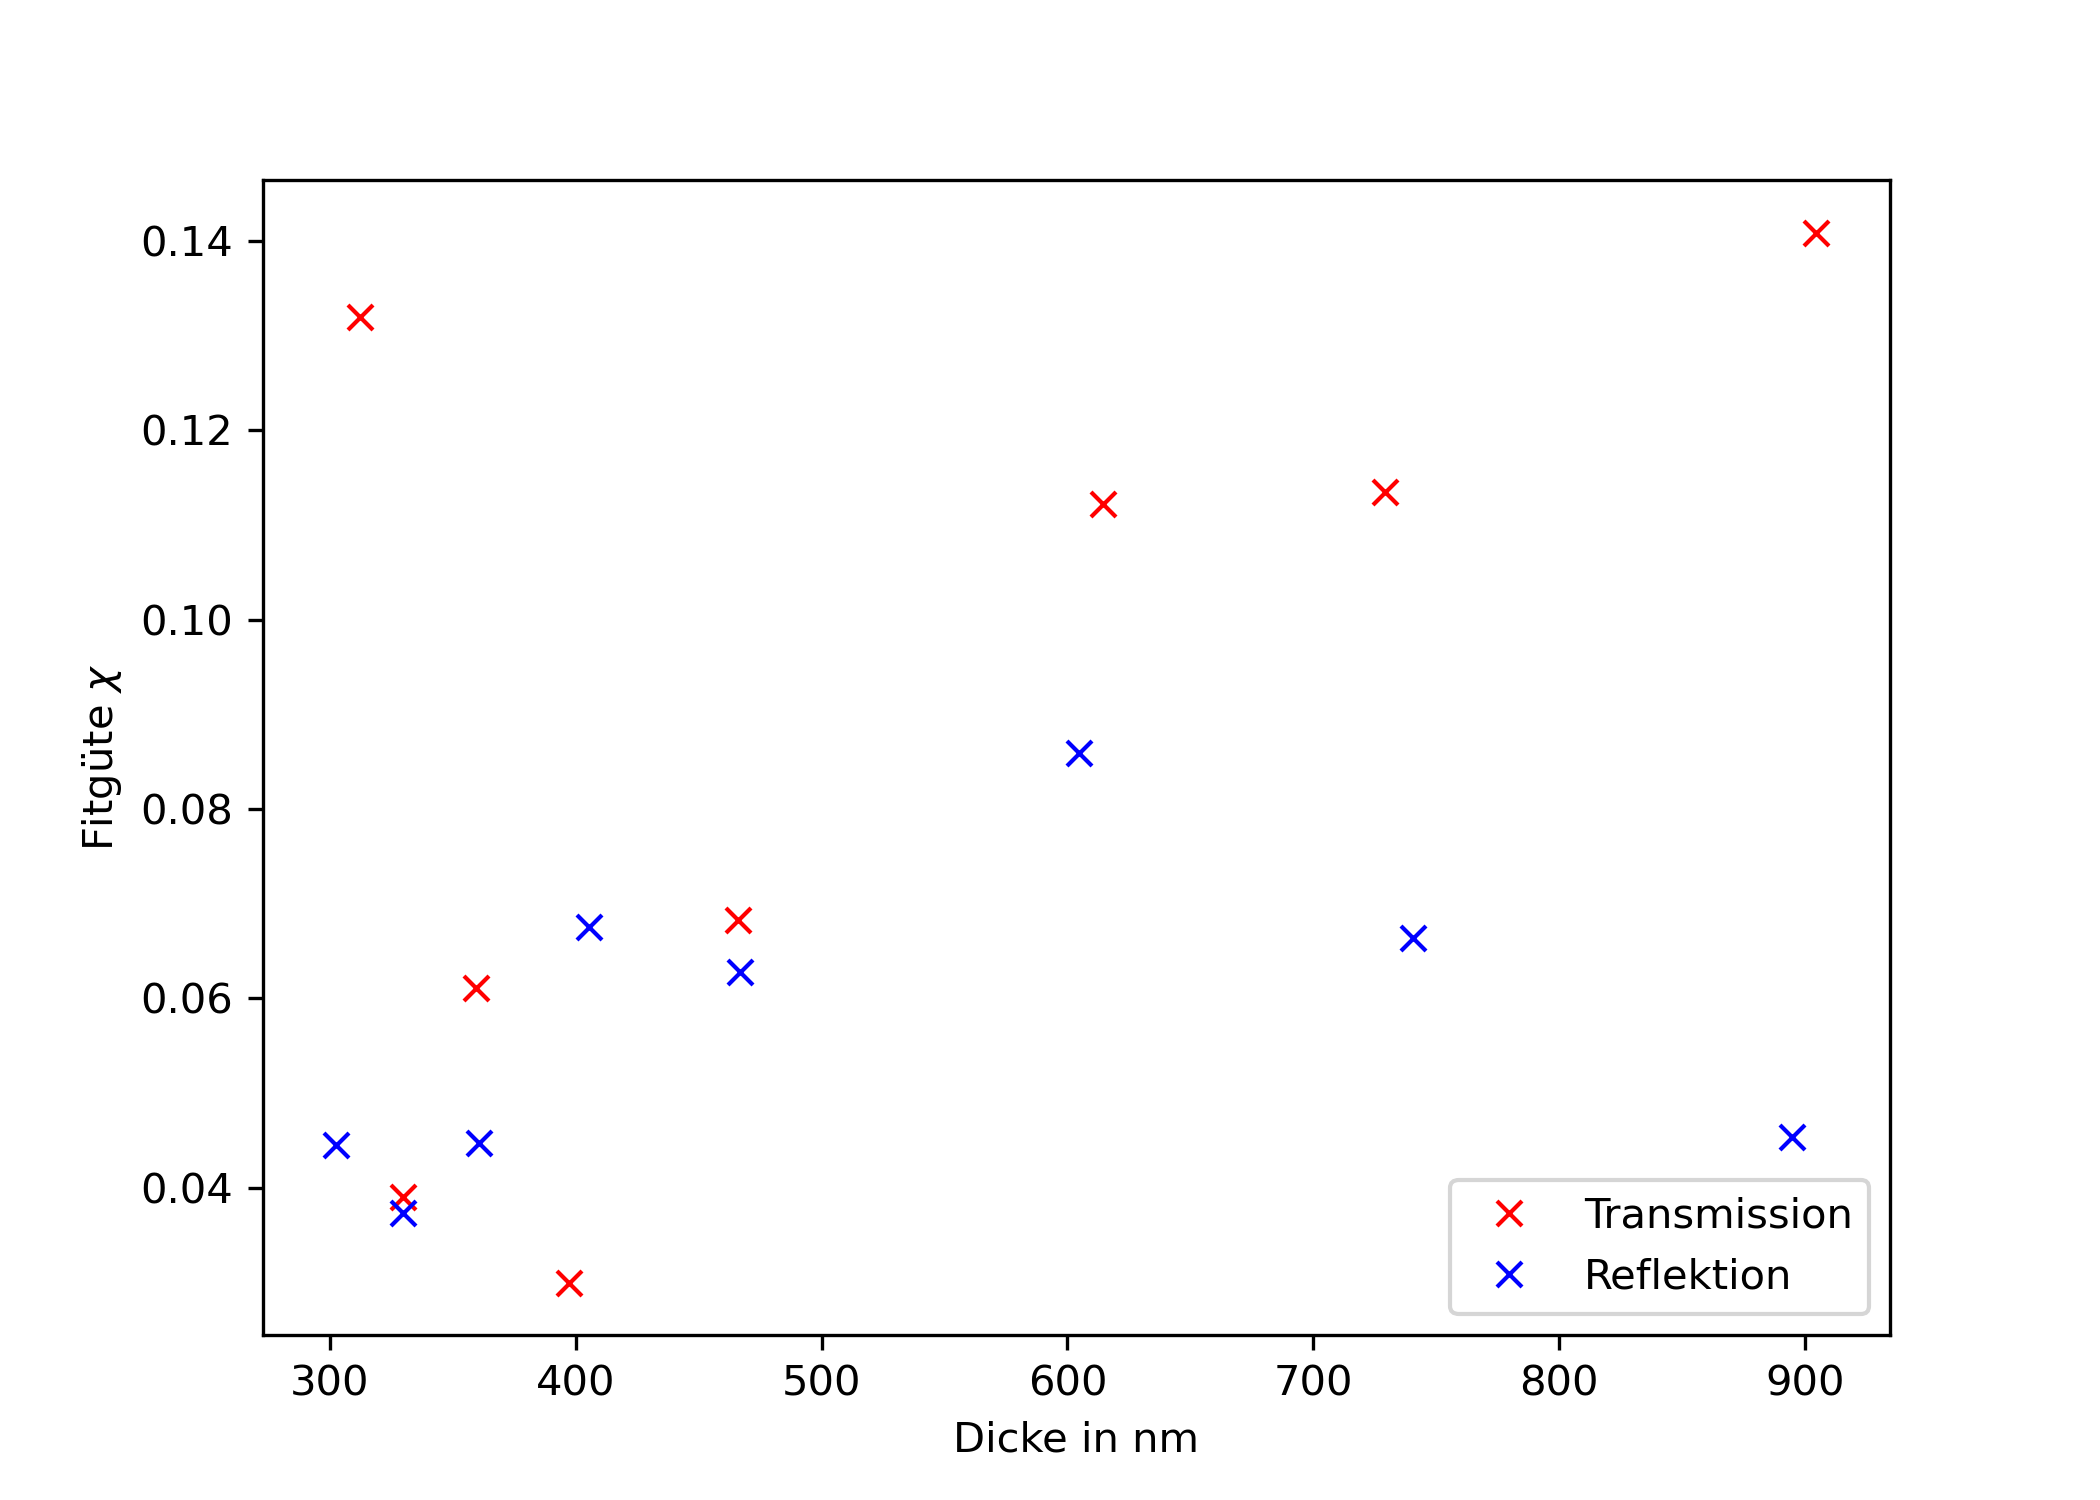
\includegraphics[width=\linewidth]{guete_dicke_rpm.png}
    \caption{Variable Rotationsgeschwindigkeit.}
    \label{fig:guete_rpm}
  \end{subfigure}%
  \begin{subfigure}{.4\textwidth}
    \centering
    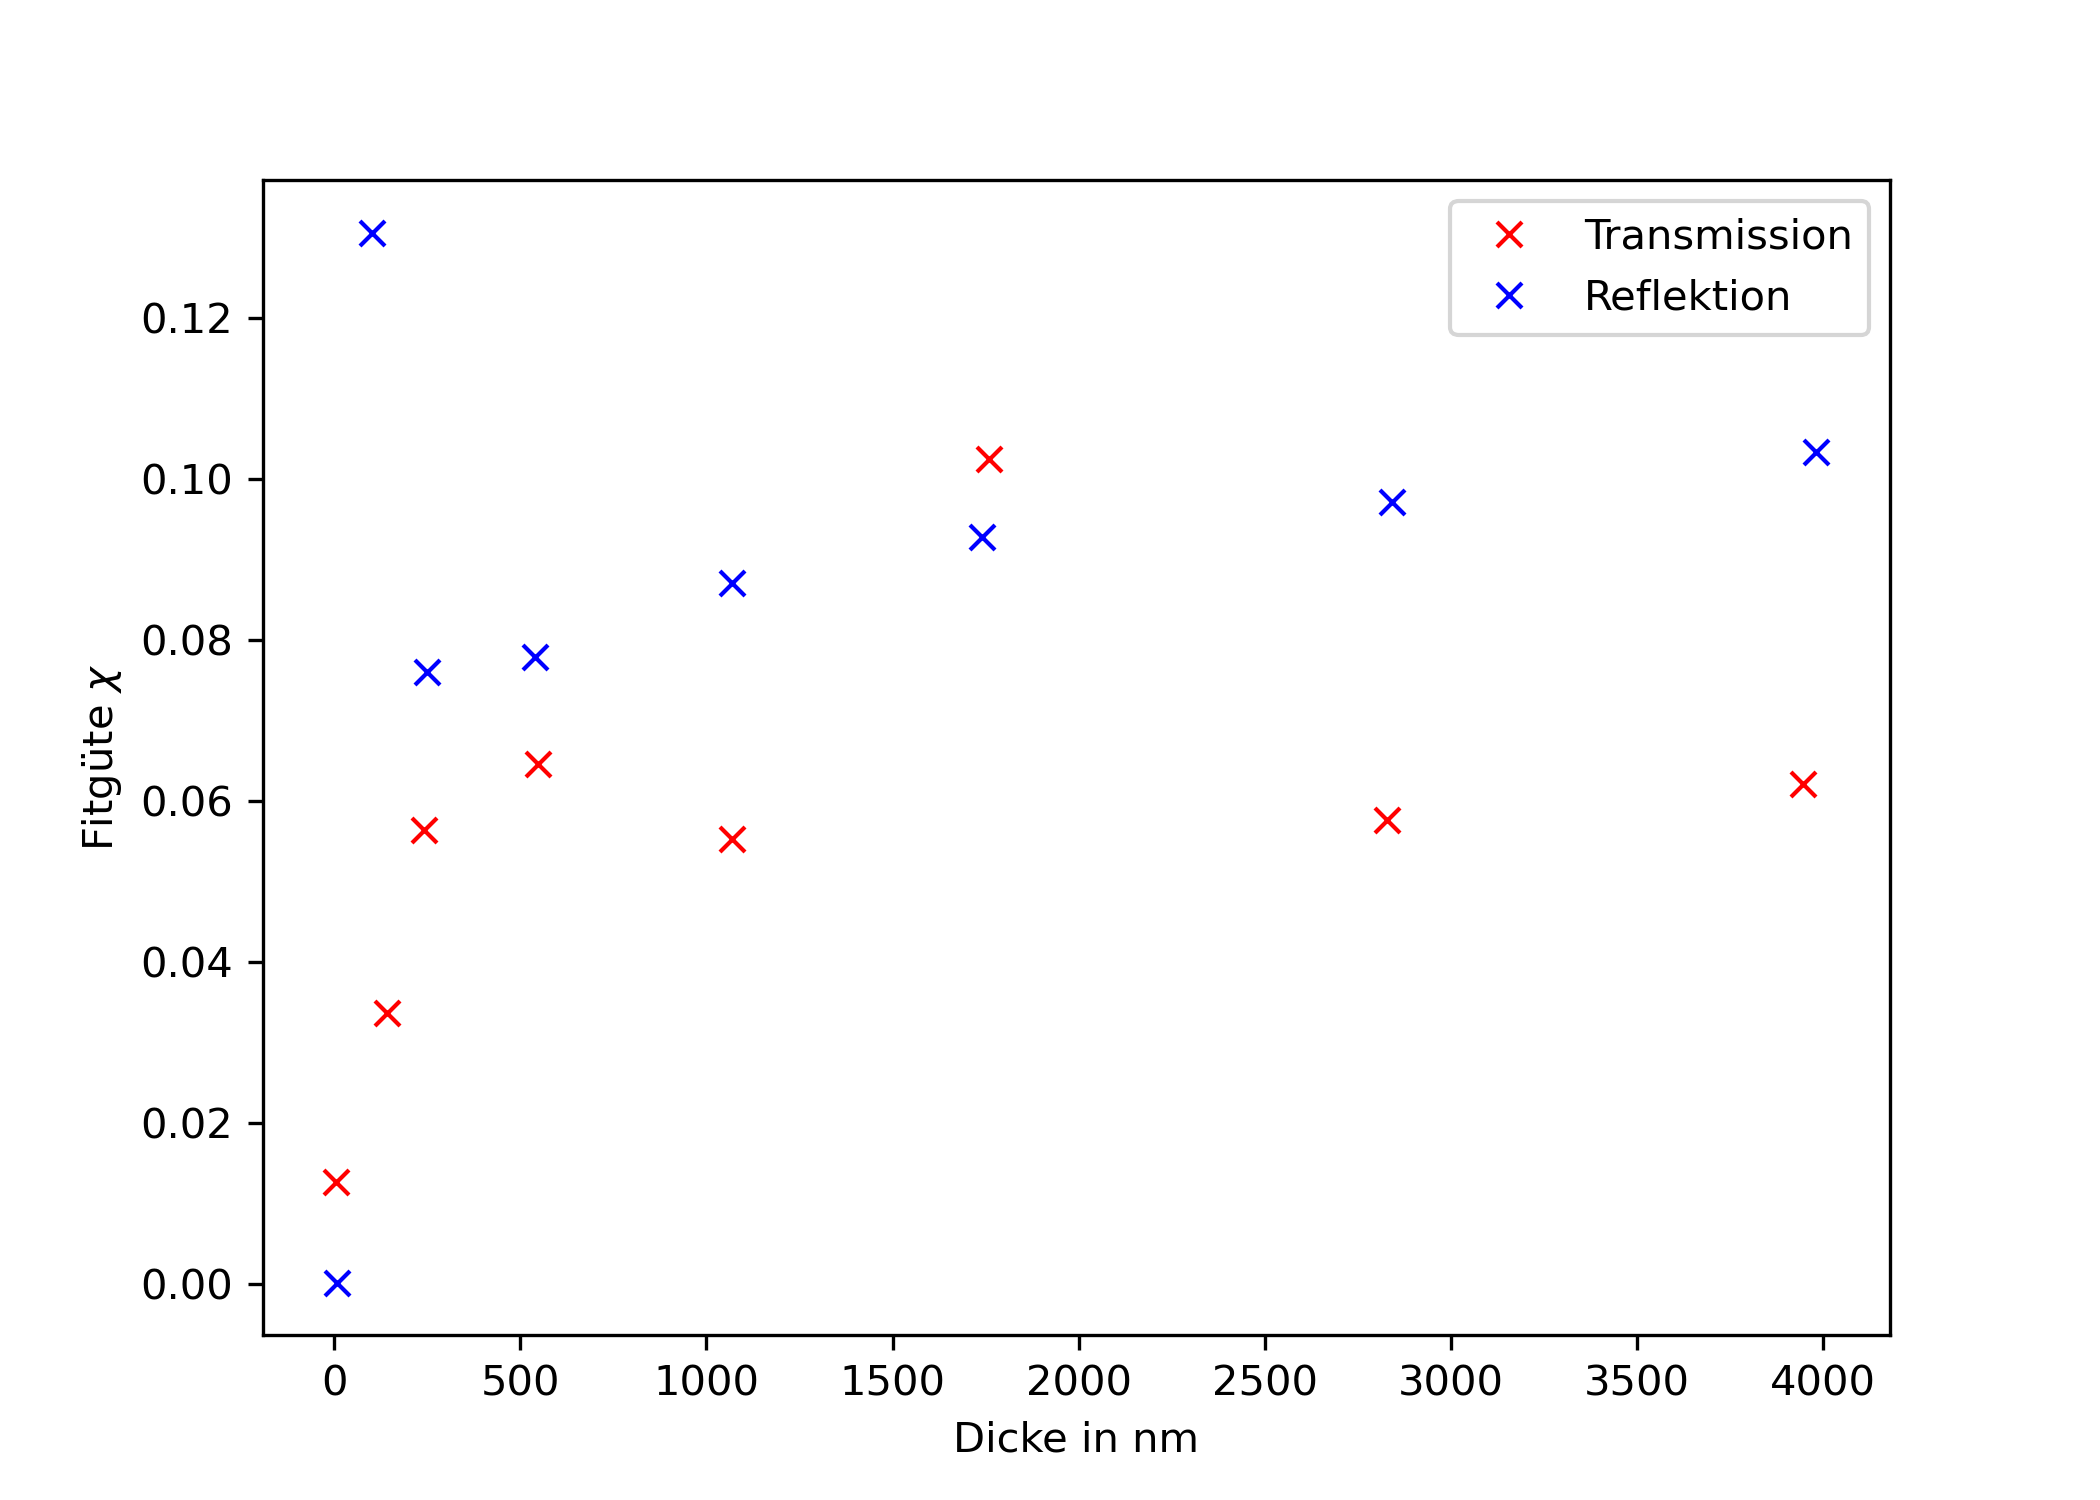
\includegraphics[width=\linewidth]{guete_dicke_conc.png}
    \caption{Variable Konzentration.}
    \label{fig:guete_conc}
  \end{subfigure}
  \caption{Schichtgüte gegen Schichtdicke für die verschiedenen Messungen. Blau sind die Reflektions-, rot die Transmissionsmessungen.}
  \label{fig:guete_spektren}
\end{figure}

Bei einer Veränderung der Rotationsgeschwindigkeit scheint die Fitgüte bei den Transmissionsmessungen höher zu sein, bei Veränderung der Konzentrationen eher andersherum, wenn auch weniger deutlich. Insgesamt lässt sich keine messmethode als klar besser identifizieren.